
\documentclass{article} % For LaTeX2e
\usepackage{iclr2023_conference,times}

% Optional math commands from https://github.com/goodfeli/dlbook_notation.
\input{math_commands.tex}

\usepackage{hyperref}
\usepackage{url}

% Recommended, but optional, packages for figures and better typesetting:
\usepackage{microtype}
\usepackage{graphicx}
% \usepackage{subfigure}
\usepackage{booktabs} % for professional tables


\usepackage[utf8]{inputenc} % allow utf-8 input
\usepackage[T1]{fontenc}    % use 8-bit T1 fonts
\usepackage{hyperref}       % hyperlinks
\usepackage{url}            % simple URL typesetting
\usepackage{booktabs}       % professional-quality tables
\usepackage{amsfonts}       % blackboard math symbols
\usepackage{nicefrac}       % compact symbols for 1/2, etc.
\usepackage{microtype}      % microtypography

\usepackage{algorithm}
\usepackage{algorithmic}
\usepackage{graphicx}
% \usepackage{subfigure}
\usepackage{xcolor}
\usepackage{comment}
\usepackage{caption}
\usepackage{subcaption}
\usepackage{amsmath}


\title{Group-Disentangling Conditional Shift}

% Authors must not appear in the submitted version. They should be hidden
% as long as the \iclrfinalcopy macro remains commented out below.
% Non-anonymous submissions will be rejected without review.

\author{Dan Andrei Iliescu \& Damon J. Wischik \thanks{ Use footnote for providing further information
about author (webpage, alternative address)---\emph{not} for acknowledging
funding agencies.  Funding acknowledgements go at the end of the paper.} \\
Department of Computer Science\\
University of Cambridge\\
Pittsburgh, PA 15213, USA \\
\texttt{\{hippo,brain,jen\}@cs.cranberry-lemon.edu} \\
\And
Ji Q. Ren \& Yevgeny LeNet \\
Department of Computational Neuroscience \\
University of the Witwatersrand \\
Joburg, South Africa \\
\texttt{\{robot,net\}@wits.ac.za} \\
\AND
Coauthor \\
Affiliation \\
Address \\
\texttt{email}
}

% The \author macro works with any number of authors. There are two commands
% used to separate the names and addresses of multiple authors: \And and \AND.
%
% Using \And between authors leaves it to \LaTeX{} to determine where to break
% the lines. Using \AND forces a linebreak at that point. So, if \LaTeX{}
% puts 3 of 4 authors names on the first line, and the last on the second
% line, try using \AND instead of \And before the third author name.

\newcommand{\fix}{\marginpar{FIX}}
\newcommand{\new}{\marginpar{NEW}}
\newcommand{\todo}[2]{\paragraph{\textcolor{red}{#1}} \textcolor{red}{#2}}
\newcommand{\add}[1]{\textcolor{red}{#1}}

%\iclrfinalcopy % Uncomment for camera-ready version, but NOT for submission.
\begin{document}


\maketitle

\begin{abstract}
We propose a novel group disentanglement method called the Context-Aware Variational Autoencoder (CxVAE). Our model can learn disentangled representations on datasets with conditional shift. This phenomenon occurs when the conditional distribution of the instance-level latent variable $\mathbf{z}$ given the input observation $\mathbf{x}$ changes from one group to another (i.e. $p_i(\mathbf{z}|\mathbf{x}) \neq p_j(\mathbf{z}|\mathbf{x})$, where $i,j$ are two different groups). We show that existing methods fail to learn disentangled representations under this scenario because they infer the group $\mathbf{u}$ and instance $\mathbf{z}$ variables separately. CxVAE overcomes this limitation by conditioning the instance inference on the group variable $q(\mathbf{z}|\mathbf{x},\mathbf{u})$. Our model has the novel ability to disentangle ambiguous observations (those with incomplete information about the generative factors), which we evaluate on the task of fair comparisons between student test scores. Additionally, we demonstrate empirically that conditional shift is the cause of our model's improved performance.
\end{abstract}

\section{Introduction}
\label{intro}

Group disentanglement is the goal of learning representations that separate group-level variation from instance-level variation. Consider a dataset of observations organised into $N$ groups of the form $\mathbf{x}_{n,1:K_n} = \{\mathbf{x}_{n,1}, ..., \mathbf{x}_{n,K_n}\}, ~ n \in 1:N$. These could be pictures grouped by author, clinical outcomes grouped by the patient, or film ratings grouped by user.  We train a representation network $r(\mathbf{x}_n)$ that encodes a group of observations $\{\mathbf{x}_{n, 1}, \dots \mathbf{x}_{n,K_n}\}$ into one group code $\mathbf{u}_n$ and a set of instance codes $\{\mathbf{z}_{n,1}, \dots \mathbf{z}_{n, K_n}\}$, one for each observation. We want $\mathbf{u}$ to capture only the variation across groups and $\mathbf{z}$ only the variation within groups. 

The current state-of-the-art approaches for group disentanglement train the representation network $r$ by using it as the variational latent posterior distribution in a Variational Autoencoder \citep{Bouchacourt2018MultiLevelVA, Hosoya2019GroupbasedLO, Nmeth2020AdversarialDW}. They assume a hierarchical generative model whereby the observation $\mathbf{x}_{n,k}$ is generated by combining a group latent variable $\mathbf{u}_n$ and an independent instance latent variable $\mathbf{z}_{n,k}$ (Figure~\ref{fig:pgm}-left). The standard setup involves training the variational latent posterior $q(\mathbf{u}_n, \mathbf{z}_{n,1:K_n} | \mathbf{x}_n)$ by maximising a lower bound to the data likelihood \citep{Kingma2014AutoEncodingVB, JimenezRezende2014StochasticBA}. 

In our work, we show that the variational latent posterior, as conceived in existing models, is unsuited to datasets with \textit{conditional shift}. This is a property of the data-generating process whereby the true conditional distribution of the instance latent variable $\mathbf{z}$ changes from one group to another $p_i(\mathbf{z} | \mathbf{x}) \neq p_j(\mathbf{z} | \mathbf{x})$ where $i,j$ are two groups \citep{Zhang2013DomainAU, Gong2016Domain}. In our case, the conditional instance distribution for group $i$, which is $p_i (\mathbf{z} | \mathbf{x})$, corresponds to $p(\mathbf{z}_{i,k} | \mathbf{x}_{i,k}, \mathbf{u}_i)$ where $k$ is a given instance in the group.

Conditional shift occurs in many real-world datasets that we would like to group-disentangle. For example, in the context of collaborative filtering, if we want to infer the quality of an item based on a user rating, we should take into account how the same user rated other items \citep{Koren2009MatrixFT}. Different users might give the same rating to items of different quality based on their preferences, so inferring the item representation without conditioning on the user will produce widely varying estimates across users \citep{Pinheiro2001MixedEffectsMI}.

\begin{figure}[th]
    \vskip 0.2in
    \begin{center}
    \centerline{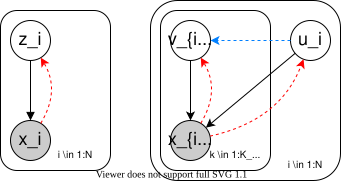
\includegraphics[width=\columnwidth]{files/bayes_net.pdf}}
    \caption{\textbf{Our variational distribution conditions the instance representation $\mathbf{z}_{n,k}$ on the group representation $\mathbf{u}_n$.} Group-instance generative model (\textbf{left}). Variational model of the GVAE (\textbf{middle}). Our conditional variational model (\textbf{right}).}
    \label{fig:pgm}
    \end{center}
    \vskip -0.2in
\end{figure}

Existing VAE-based methods fail to disentangle in the conditional shift setting because they make the assumption that the group and instance variables can be inferred independently of each other from the input observation (Figure \ref{fig:pgm}-middle):
When defining the variational latent posterior, existing works based on the Group VAE (GVAE) \citep{Bouchacourt2018MultiLevelVA, Hosoya2019GroupbasedLO, Nmeth2020AdversarialDW, Chen2020WeaklySD} make the assumption that the group and instance variables are conditionally independent given the observations (Figure \ref{fig:pgm}-middle):

\begin{equation}
\label{eq:indep}
q(\mathbf{u}_n, \mathbf{z}_{n,1:K_n} | \mathbf{x}_{n,1:K_n}) = q(\mathbf{u}_n | \mathbf{x}_{n,1:K_n}) \sum_{k=1}^{K_n} q(\mathbf{z}_{n,k} | \mathbf{x}_{n,k}).
\end{equation}

The limitations of this assumption have not been identified so far in the literature because the datasets used to test disentanglement,  such as Shapes3D \citep{Kim2018DisentanglingBF}, SmallNORB \citep{LeCun2004LearningMF}, dSprites \citep{Higgins2017betaVAE}, Cars3D \citep{Reed2015DeepVA}, MPI3D \citep{Gondal2019OnTT}, have the property that one image is always sufficient to accurately infer its latent variables. For example, we only require a single image from the MPI3D dataset to uniquely identify the colour, position, and rotation of the depicted object.

We present the following contributions:

\begin{enumerate}
\item We show that even a simple dataset with conditional shift can prohibit current methods from learning disentangled representations (Figure \ref{fig:trans_theirs}).  We approach the task of learning fair representations of students from different schools/socio-economic backgrounds. 
\item We propose a new model, the Context-Aware VAE (CxVAE), that has the ability to produce group-disentangled representations of datasets with conditional shift (Figure \ref{fig:trans_ours}). 
\item We show that conditional shift directly causes our model's improvement in performance over existing methods.
\end{enumerate}

\begin{figure}[t]
\vskip 0.2in
\begin{center}
\begin{subfigure}[t]{0.32\linewidth}
\includegraphics[width=\textwidth]{files/data_data.pdf}
\caption{Test scores grouped by school.}
\label{fig:data}
\end{subfigure}
\hfill
\begin{subfigure}[t]{0.32\linewidth}
\includegraphics[width=\textwidth]{files/trans_theirs.pdf}
\caption{Failed translation (GVAE).}
\label{fig:trans_theirs}
\end{subfigure}
\hfill
\begin{subfigure}[t]{0.32\linewidth}
\includegraphics[width=\textwidth]{files/trans_ours.pdf}
\caption{Successful translation (ours).}
\label{fig:trans_ours}
\end{subfigure}
\caption{\textbf{Our model correctly disentangles between student aptitude and school characteristics, whereas the GVAE \citep{Hosoya2019GroupbasedLO} fails.} We ask the counterfactual question ``What score would student $k$ from school $A$ have obtained if they had attended the \textit{typical school}?''. The task is to generate a set of test scores by translating the scores from school $A$ onto the distribution of scores from the typical school. Each line shows the translation for an individual student. Our model preserves the relative positions of the scores, whilst also capturing the distribution of the typical school.}
\label{fig:trans}
\end{center}
\vskip -0.2in
\end{figure}

\section{Related Work}

\paragraph{Group Disentanglement.} This class of problems comes under different names: style-content disentanglement \citep{Tenenbaum2000SeparatingSA}, content-transformation disentanglement \citep{Hosoya2019GroupbasedLO},  and disentanglement with group supervision \citep{Shu2020Weakly}, to name a few. Recent work \citep{Shu2020Weakly, Locatello2020WeaklySupervisedDW} has contextualised GID as a subproblem of weakly-supervised disentanglement, where disentangled representations are learned with the help of non-datapoint supervision (e.g. grouping, ranking, restricted labelling). Early work in this area focused on separating between visual concepts \citep{Kulkarni2015DeepCI, Reed2015DeepVA}. This area has received renewed interest after the theoretical impossibility result of \citet{Locatello2019ChallengingCA} and the identifiability proofs of \citet{Khemakhem2020VariationalAA} and \citet{Mita2021AnID}. A key aspect of recent weakly-supervised models is the interpretation of the grouping as a signal of similarity between datapoints \citep{Chen2020WeaklySD}. 

\paragraph{Conditioning on the Group Variable.} While conditioning the instance encoder on the group variable is common in the areas of semi-supervised learning and fair representations \citep{Kingma2014Semisupervised, Louizos2016TheVF}, we are the first to apply it to unsupervised group disentanglement where explicit group labels are not available. In the field of sequence disentanglement, state-of-the-art methods \citep{Hsu2017UnsupervisedLO, Denton2017UnsupervisedLO, Li2018DisentangledSA} infer the instance variable (capturing shorter timescales) conditionally on the group variable (capturing longer timescales). Recent works in weakly-supervised disentanglement \citep{Shu2020Weakly, Locatello2019ChallengingCA, Roeder2019Efficient} also condition the instance variable on the group, but their group variable is a discrete variable used for selection rather than a representation. It marks which units of the instance representation are common within the group and which are free to vary. We argue that this is not sufficient to account for the variation in $p(v | x, u)$ produced by the conditional shift, so we include AdaGVAE \citep{Locatello2020WeaklySupervisedDW} in our evaluation for comparison (see Section~\ref{sec:results}).

\paragraph{Conditional Shift} Our instance encoder conditioned on the group variable is a new strategy to deal with conditional shift. This problem has been studied extensively in the context of supervised learning \citep{Zhang2013DomainAU, Gong2016Domain}. Methods for mitigating the effects of conditional shift typically focus on learning domain-invariant representations \citep{BenDavid2009A}. However, \citet{Zhao2019On} show that learning a domain-invariant representation is not sufficient for learning a correct mapping between instance variables from different groups.

\paragraph{Image Translation.} Note that our variational latent posterior is different from the one used in COCO-FUNIT \citep{Saito2020Coco}. The authors are motivated by the same limitations with existing works as we are, namely that unsupervised translation methods struggle to disentangle under conditional shift. However, because they train explicitly for translation rather than disentanglement, they arrive at a different solution than ours. When performing a translation, their approach is to condition the representation of the target group on the source image, thereby bypassing the need for an accurate instance representation. This mechanism produces impressive results on image translation tasks, but it cannot be extended to models based on the GVAE which do not train explicitly for translation; in our case, there are no source and target groups in the training set. Regardless, we evaluate COCO-FUNIT on the test score dataset and show that our model outperforms it both in terms of disentanglement and translation.

\section{Background}

\subsection{Fair Comparisons Between Students}

Consider the task of fair comparisons between students attending different schools based on their standardised test scores in maths and reading \citep{Braun2006ComparingPS}. The typical assumption in the literature is that each school has a similar distribution of aptitude among its students, so our goal is to learn disentangled student-level (instance) and school-level (group) representations of the scores. The instance representation $\mathbf{z}_{n,k}$ should reflect the aptitude of student $k$ from school $n$ independently of what school the student had attended.

This analysis is crucial for university admission boards aiming to judge students based on their aptitude regardless of the socio-economic circumstances associated with attending one school or another, such as affluence, location, or curriculum \citep{Raudenbush1995TheEO, Braun2006ComparingPS}. Group disentanglement has the potential to reduce the computational costs of this analysis compared to the current variational inference methods for mixed-effects models \citep{Gelman2006Data}. The variational latent posterior of a GVAE can perform scalable inference of the student and school representations requiring just one forward pass through the network for every additional student. Contrast this with running a separate optimisation routine for the latent variables of each student \citep{Gelman1995BayesianDA}. GVAEs can also optimise highly non-linear generative models which would otherwise have to be designed explicitly for the problem in hand \citep{Pinheiro2001MixedEffectsMI}.

Current methods fail to learn disentangled representations on this data. Figure \ref{fig:trans_theirs} shows the GVAE model \citep{Hosoya2019GroupbasedLO} incorrectly translating the scores from one school to another. Translation is a well-established downstream task for evaluating disentanglement \citep{Tenenbaum2000SeparatingSA}. In the case of test scores, translation corresponds to the counterfactual question ``What score would student $k$ from school $A$ have obtained if they had attended the \textit{typical school} (i.e. a school whose scores are distributed according to $\mathcal{N}(0,I_2)$)?''. We do this by generating a new score by combining the instance representation of student $k$ from school $n$ with the group representation of the typical school. \citet{Raudenbush1995TheEO} use translation to directly compare students from different schools. Notice that the unconditional GVAE scrambles the order of the scores and fails to capture the $\mathcal{N}(0,I_2)$ distribution of the typical school.

% \com{Move to higher priority}

We propose a modification to the variational latent posterior in order to enable the GVAE to learn disentangled representations of test score data. Looking at the data (Figure \ref{fig:data}), it is clear that we are dealing with the conditional shift scenario. The same reading score could be obtained by either a high-achieving student from school $C$ or a low-achieving student from school $B$. Inferring the aptitude of the student requires knowing the distribution of scores within each school. In order to account for the variation across groups, we introduce the Context-Aware Variational Autoencoder (CxVAE), whose instance encoder is conditioned on the group representation (Figure~\ref{fig:pgm}-right). This reflects the correct factorisation of the generative latent posterior $p(\mathbf{u}_n, \mathbf{z}_{n,1:K_n} | \mathbf{x}_{n,1:K_n})$, thus making no assumptions about the relationship between the group and the instance. We observe our variational model successfully translating test scores in Figure~\ref{fig:trans_ours}.

\subsection{Group-Instance Generative Model}

The Group-Instance Generative Model \citep{Bouchacourt2018MultiLevelVA,Hosoya2019GroupbasedLO} is a multi-level model that uses two latent variables to generate grouped data: the instance variable $\mathbf{z}_{n,k} \sim \mathcal{N} (0,1)$ controls the variation within groups, and the group variable $\mathbf{u}_n \sim \mathcal{N} (0, 1)$ controls the variation across groups (Figure~\ref{fig:pgm}-left). The likelihood of a group $\mathbf{x}_{n,1:K_n}$ is:

\begin{equation}
p(\mathbf{x}_{n, 1:K_n}) = \mathbb{E}_{p(\mathbf{u}_n)}  \prod_{k=1}^{K_n} \mathbb{E}_{p(\mathbf{z}_{n,k})} ~ [p(\mathbf{x}_{n,k} | \mathbf{u}_n, \mathbf{z}_{n,k})]
\end{equation}

\subsection{Variational Inference}

Because the exact likelihood is intractable, the standard approach to train the group-instance generative model is with a Variational Autoencoder \citep{Kingma2014AutoEncodingVB,JimenezRezende2014StochasticBA} which performs optimisation by introducing a variational latent posterior $q(\mathbf{u}_n, \mathbf{z}_{n, 1:K_n} | \mathbf{x})$ and maximizing the Evidence Lower Bound \citep{Jordan2004AnIT}:

\begin{align}
\log p(\mathbf{x}_{n,1:K_n}) \geq ~ & \mathbb{E}_{q(\mathbf{u}_n, \mathbf{z}_{n, 1:K_n} | \mathbf{x}_{n, 1:K_n} )} \left[\sum_{k=1}^{K_n} \log p(\mathbf{x} | \mathbf{u}, \mathbf{z})\right] \\ &- \mathrm{KL} [q(\mathbf{u}_n, \mathbf{z}_{n, 1:K_n}  | \mathbf{x}_{n, 1:K_n} ) || p(\mathbf{u}_n, \mathbf{z}_{n, 1:K_n} )]
\end{align}

Existing methods use a class of variational distributions that assume conditional independence between the latent variables.

\begin{equation}
q(\mathbf{u}_n, \mathbf{z}_{n, 1:K_n}  | \mathbf{x}_{n, 1:K_n} ) = q(\mathbf{u}_n | \mathbf{x}_{n, 1:K_n} ) \prod_{k=1}^{K_n} q(\mathbf{z}_{n,k} | \mathbf{x}_{n,k})
\end{equation}

\section{Context-Aware Variational Autoencoder}

We propose a new model which can perform well on group-confounded problems. We call our model the Context-Aware Variational Autoencoder (CxVAE). Its defining feature is a variational latent posterior whose instance variable is conditioned on the group variable:

\begin{equation}
q(\mathbf{u}_n, \mathbf{z}_{n, 1:K_n}  | \mathbf{x}_{n, 1:K_n} ) = q(\mathbf{u}_n | \mathbf{x}_{n, 1:K_n} ) \prod_{k=1}^{K_n} q(\mathbf{z}_{n,k} | \mathbf{x}_{n,k},  \mathbf{u}_n)
\end{equation}

Thus, the instance encoder is implemented as a network which takes as input the concatenation of the observation $\mathbf{x}_{n,k}$ and previously sampled group representation $\mathbf{u}_n$.

\begin{equation}
q(\mathbf{z}_{n,k} | \mathbf{x}_{n,k}, \mathbf{u}_n) = \mathcal{N} (\mu, \sigma), ~~~ (\mu, \sigma) = f (\mathbf{x}_{n,k}, \mathbf{u}_n),
\end{equation}

This form of the variational distribution reflects the correct factorisation of the generative model. It has the potential to learn the true generative latent posterior, which is disentangled by definition. The Evidence Lower Bound for our model is

\begin{align}
& \mathbb{E}_{q(\mathbf{u}_n, \mathbf{z}_{n, 1:K_n} | \mathbf{x}_{n, 1:K_n})} \left[\sum_{k=1}^{K_n} \log p(\mathbf{x}_{n,k} | \mathbf{u}_n, \mathbf{z}_{n,k})\right] \\ & - \mathrm{KL} [q(\mathbf{u}_n| \mathbf{x}_{n,1:K_n}) || p(\mathbf{u}_n)] \\ & - \mathbb{E}_{q(\mathbf{u}_n | \mathbf{x}_{n,1:K_n})}\left[\sum_{k=1}^{K_n} \mathrm{KL}[q(\mathbf{z}_{n,k} | \mathbf{x}_{n,k},\mathbf{u}_n) || p(\mathbf{z}_{n,k})]\right].
\end{align}

\section{Methodology}

We show that by making the instance encoder conditional on the inferred group variable, we obtain a considerable gain in translation accuracy and a marked improvement in disentanglement. We also demonstrate that the gap in performance between our model and other group disentanglement methods is caused by conditional shift in the data-generating process.

\subsection{Setup}
\label{sec:setup}

We compare our conditional CxVAE with the state-of-the-art in group disentanglement, namely the Group VAE \citep{Hosoya2019GroupbasedLO, Bouchacourt2018MultiLevelVA}, COCO-FUNIT \citep{Saito2020Coco}, and AdaGVAE \citep{Locatello2019ChallengingCA}. We implement all networks (encoders and decoders) as MLPs with 3 hidden layer of 32 activations each. As in \citet{Hosoya2019GroupbasedLO}, the group encoder is applied to each datapoint in the group and then all the outputs are averaged. The group variable will have 4 dimensions (2 for $\mathbf{b}_n$ and 2 for $\mathbf{c}_n$) and the instance variable will have 2 dimension (for $\mathbf{a}_{n,k}$). 

For all experiments, our CxVAE will be a modified GVAE such that the group variable $\mathbf{u}_n$ is concatenated with the observation $\mathbf{x}_{n,k}$ and fed into the instance encoder in order to compute the instance variable $\mathbf{z}_{n,k}$.

We train each model for 64 epochs, and use the last 10 epochs for evaluation. Additionally, we run the experiment for 100 different random seeds initialisations, both for the data generating process and the networks. We use the same 100 seeds in each model. This gives 1000 measurements to plot in Figure~\ref{fig:results}. Training and testing take approximately 2 hours to run on an Intel i9 CPU.

\subsection{Dataset}
\label{sec:dataset}

We generate our dataset of test scores using the classic ``varying intercept, varying slope'' mixed-effects model \citep{Laird1982Random, Pinheiro2001MixedEffectsMI, Gelman2006Data}. This is a well-established approach for modelling student scores $\mathbf{x}_{n,k}$ as a function of individual aptitude $\mathbf{a}_{n,k}$ and school-level characteristics $(\mathbf{b}_n, \mathbf{c}_n)$ (e.g. affluence, curriculum, location, etc.) \citep{Raudenbush1995TheEO, Braun2006ComparingPS}. We choose this model for its simplicity and for the wide variety of phenomena to which it can be applied. All the scores and factors are 2-dimensional vectors, with one component for the maths score and another for the reading score:

\begin{align} \label{eq:score}
& \mathbf{x}_{n,k} = \mathbf{b}_n - \mathbf{c}_n \odot \mathbf{a}_{n,k} + \epsilon_{n,k} ~~ \text{is the score of student} ~ k ~ \text{in school} ~ n.\\
& \mathbf{a}_{n,k} \sim \mathcal{N} (0,I_2) ~~ \text{is the aptitude of student} ~ k ~ \text{in school} ~ n\\
& \mathbf{b}_n \sim \mathcal{N} (0,I_2) ~~ \text{is the mean score in school } n\\
& \mathbf{c}_n \sim \mathrm{Exp} (1) ~~ \text{is the standard deviation of scores in school } n\\
& \epsilon_{n,k} \sim \mathcal{N} (0, 0.1 * I_2) ~~ \text{is a per-student error term.}
\end{align}

For the evaluation procedure, we use the above model to generate $N=32,768$ values for $\mathbf{b}_n, \mathbf{c}_n$. For each school $n$, we generate $M=128$ values for $\mathbf{a}_{n,k}$. We then randomly select half of the schools to assemble a training dataset with $2,097,152$ scores split across $16,384$ schools. We take the other half of schools to create the holdout dataset, so that every testing school and student are unseen during training. 

We have chosen to evaluate on a synthetic dataset because it allows for fine control over the parameters of the data-generating process (especially relevant in Section~\ref{sec:xy}) and it also enables us to measure the quality of disentanglement using the Mutual Information Gap \citep{Chen2018IsolatingSO}.

\subsection{Metrics}

\begin{figure}[t]
\vskip 0.2in
\begin{center}
\centerline{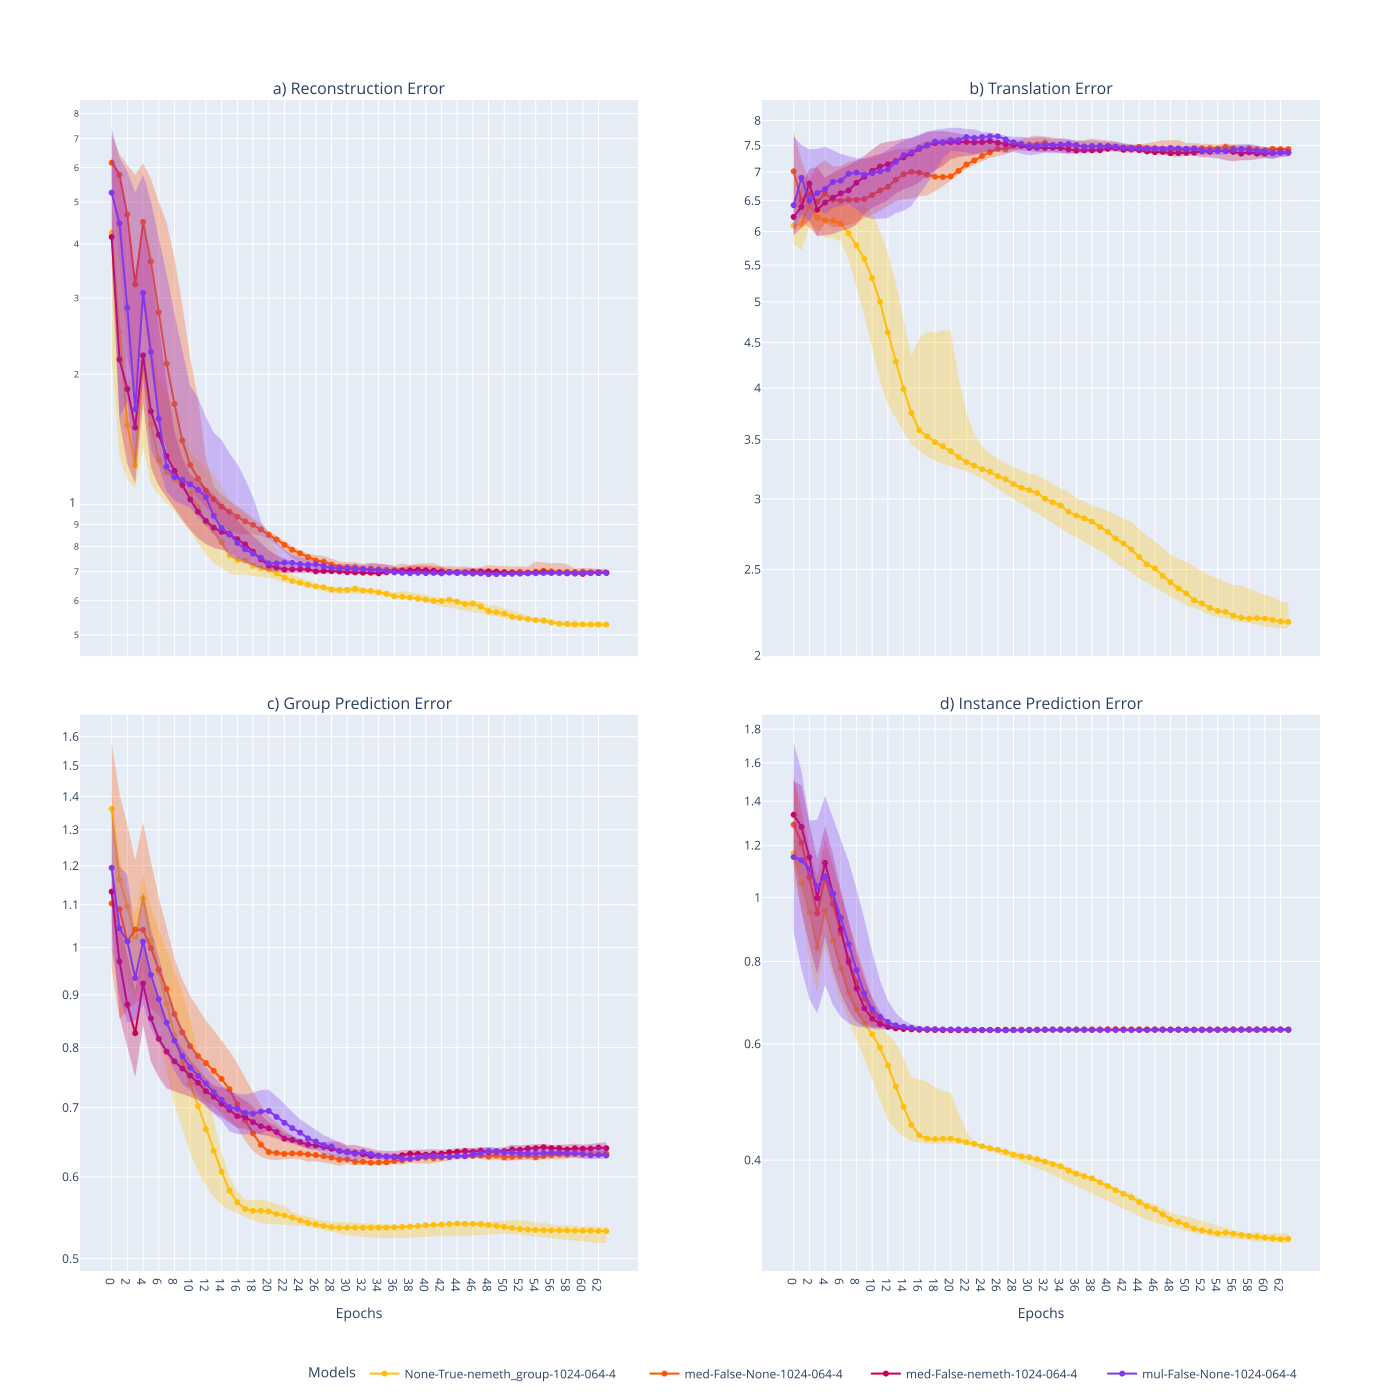
\includegraphics[width=\columnwidth]{files/results.pdf}}
\caption{Our CxVAE produces considerable improvements over the state-of-the-art in every metric considered: holdout reconstruction error (\textbf{lower is better}), translation error (\textbf{lower is better}), MIG disentanglement score (\textbf{higher is better}).}
\label{fig:results}
\end{center}
\vskip -0.2in
\end{figure}

We compare the models with respect to 3 different criteria: 1) How well does the model fit the holdout data?, 2) How disentangled are the representations inferred by the encoder?, and 3) How well can the model answer the counterfactual question "What score would a student have obtained if they had gone to a different school?". We assess each criterion with a different evaluation metric.

\paragraph{Fitting the holdout data.} As a general metric, we report the reconstruction error (MSE) on the holdout data for every experiment, commonly used as a proxy for the likelihood of the holdout set.

\paragraph{Disentangled representations.} We use the Mutual Information Gap \citep{Chen2018IsolatingSO} to measure the quality of the disentanglement. We measure empirically the amount of mutual information between the inferred latent variables $\mathbf{u},  \mathbf{z}$ and the school characteristics $(\mathbf{b}, \mathbf{c})$ which represent the ground-truth group factor. Consequently, the goal is to have maximum mutual information between the group variable $\mathbf{u}$ and the ground-truth, and minimum mutual information between the instance variables $\mathbf{z}$ and the ground-truth.  The gap between the two (normalized with the entropy of the ground-truth factors) is the metric of disentanglement:

\begin{equation}
\mathrm{MIG} = \frac{1}{H(\mathbf{b}, \mathbf{c})} (I(\mathbf{u}; \mathbf{b}, \mathbf{c}) - I(\mathbf{z}; \mathbf{b}, \mathbf{c}))
\end{equation}

Since the data-generating process is known, the mutual information between the inferred group variable and the ground-truth group variable $I(\mathbf{u}; \mathbf{b}, \mathbf{c})$ is straightforward to implement by following the process of \citet{Chen2018IsolatingSO}.

We measure only the mutual information between the ground-truth group factor and the latent variables because,  as pointed out by \citet{Nmeth2020AdversarialDW}, the common failure case we are trying to guard against in group disentanglement is that the instance variables $\mathbf{z}$ might learn information belonging to the ground-truth group factors $(\mathbf{b}, \mathbf{c})$.

\paragraph{Counterfactual question.} We measure how well the learned representations can answer the question ``What would the score of student $k$ from school $n$ have been if they had attended the typical school (the school with scores distributed according to $\mathcal{N} (0, I_2)$)?''. This problem, also known as translation, is a commonly used downstream task for disentangled representations \citep{Tenenbaum2000SeparatingSA}. We translate the score of student $k$ to the typical school, and then take the mean squared error against the ground-truth translation, which is generated when the data is generated using the ground-truth generative factors. For our dataset, the correct translation corresponds to the Earth-Mover distance between the multivariate normal distributions of scores in each school \citep{Knott1984On}.

In order to obtain the translation, we first infer the instance variable of student $k$ from school $n$ and the group variable of the typical school. We then feed the two variables to the decoder. For evaluation, we translate all the scores from each school $n$ and then measure the distance between the predicted translation and the ground-truth translation. We compute the total error as an average over all the translation errors.

We can also use translation as an additional qualitative comparison between CxVAE and other group disentanglement methods, which can be seen in Figure~\ref{fig:trans}.

\section{Results}
\label{sec:results}

Our CxVAE produces considerable improvements over the competing methods in terms of fitting the holdout set, disentangled representations, translation accuracy and predicting the generative factors (Figure~\ref{fig:results}). While the scores of the existing methods cluster together, the gap between them and the CxVAE is larger than the 95\% confidence interval of any method.

\subsection{Conditional Shift Causes the Gap in Performance}
\label{sec:xy}

\begin{figure}[t]
\vskip 0.2in
\begin{center}
\centerline{
\includegraphics[width=\textwidth]{files/xy_ratio.pdf}}
\caption{\textbf{Conditional shift in the dataset causes the relative performance gain of our CxVAE over the GVAE.} We show performance on datasets generated with different values of the $\lambda$ hyper-parameter, controlling the amount of conditional shift. For low values of $\lambda$ the conditional distribution of student aptitude given a score changed very little from one group to another, and so the CxVAE and GVAE perform equally well. However, as $\lambda$ increases, the GVAE fails to disentangle.}
\label{fig:xy}
\end{center}
\vskip -0.2in
\end{figure}

We show, by modifying the data-generating process (\ref{eq:score}), that conditional shift explains the increased performance of the CxVAE. We insert a hyper-parameter $\lambda$ to control the strength of the conditional shift; $\lambda=1$ means the conditional shift stays the same as in the previous experiment, while $\lambda=0$ means there is no conditional shift. 

Consider the case where the maths score only depends on the school, and the reading score only depends on the student. In this situation, the two generative factors can be easily disentangled since you can infer the student aptitude from the reading score and the school profile from the maths score. We use this as an extreme case of lack of conditional shift, and insert a hyper-parameter $\lambda$ in our data-generating process that will continuously move between this case and the original case. Our modified data-generating process is

\begin{align}
& \mathbf{x}_{n,k} = \begin{bmatrix} \lambda \\ 1 \end{bmatrix} \odot \mathbf{b}_n + \begin{bmatrix} 1 \\ \lambda \end{bmatrix} \odot \mathbf{a}_{n,k} \odot \left(c_n \hat{\cdot} \begin{bmatrix} \lambda \\ 1 \end{bmatrix} \right) + \epsilon_{n,k}
\end{align}

where $\hat{\cdot}$ denotes the elementwise power operation and the generative factors $(\mathbf{a}_{n,k}, \mathbf{b}_n, \mathbf{c}_n, \epsilon_{n,k})$ are sampled as in (\ref{eq:score}).

This model has no conditional shift when $\lambda=0$ because each ground-truth factor controls a separate component of the data. Inferring the student aptitude requires only the reading score and can ignore the school characteristics. When $\lambda=1$, the problem exhibits conditional shift in exactly the same way as in (\ref{eq:score}).

If our hypothesis is correct, that the conditional shift causes the performance gap between CxVAE and other group disentanglement methods, then the gap should decrease as $\lambda$ approaches 0. The measurements displayed in Figure \ref{fig:xy} confirm our expectations. For low values of $\lambda$ the performance of our CxVAE is evenly matched to the GVAE.  As $\lambda$ increases, CxVAE metrics remain stable while GVAE performance decreases substantially.  It is clear that the degree of confounding in the dataset explains the performance gain that we see in the CxVAE. 

\section{Conclusions}
\label{sec:conclusion}

In this work, we show empirically that conditioning the instance encoder on the group variable produces group-disentangled representations on datasets with conditional shift. We also show that the strength of the conditional shift in the data-generating process determines the performance gap between our model and other group disentanglement methods. Our evaluation is run on the downstream task of extracting student aptitudes from a dataset of test scorse grouped by school, a problem on which group-instance models have not been applied before.

The main limitation of our work is that we perform evaluation on a synthetic dataset of student scores rather than real data. Although this is a justifiable choice with respect to evaluation (it gives us access to the ground-truth values of the latent variables), future work should focus on evaluating on real-world datasets with conditional shift, such as user-item ratings \citep{Koren2009MatrixFT}.

\bibliography{main}
\bibliographystyle{iclr2023_conference}

%%%%%%%%%%%%%%%%%%%%%%%%%%%%%%%%%%%%%%%%%%%%%%%%%%%%%%%%%%%%

\appendix
\section{Appendix}
You may include other additional sections here.

\end{document}
